\newpage
\section{細径McKibben型空気圧人工筋肉}
%%%%%%%%%%%%%%%%%%%%%%%%%%%%%%%%%%%%%%%%%%%%%%%%%%%%%%%%%
\subsection{McKibben型空気圧人工筋肉アクチュエータ(MPA)}
% ・今のとこは先輩のやつを真似ただけ.
MPAはシリコンゴムチューブをナイロンメッシュで覆うことで構成されており(図\ref{fig:MPA}\subref{fig:Structure}),両端に栓をするシンプルな構造である.
これに圧縮した空気を印加することでシリコンゴムチューブが膨張しメッシュによる自身の軸方向への張力が発生するアクチュエータである(図\ref{fig:MPA}\subref{fig:move}).
高出力かつ素材自体も軽量で,物理的柔軟性による高い弾性力を持つという利点があり,筋肉の代用として生物を模したロボットやリハビリなどに用いられる.
しかし図\ref{fig:MPA}に示すような従来の直径数十 mmのMPAは膨張時の径の拡大が大きいため配置の際は膨張を阻害しないような配置や直線形状で駆動するような取り付け方が求められ,取り付けの位置や密度に制限がある.
%%%%%%%%%%%%%%%%%%%%%%%%%%%%%%%%%%%%%%%%%%%%%%%%%%%%%%%%%
\begin{figure}[b]
  %
  \begin{minipage}{0.49\columnwidth}
    \vspace{4mm}
    \centering
    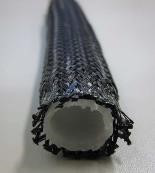
\includegraphics[scale=1]{image/MPA_kousei.png}
    \vspace{3mm}
    \subcaption{MPA断面図}
    \label{fig:Structure}
  \end{minipage}
  %
  \begin{minipage}{0.49\columnwidth}
    \vspace{25mm}
    \centering
    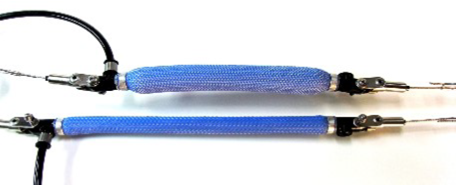
\includegraphics[scale=.8]{image/MPA_dousa.png}
    \subcaption{MPA外観および動作の様子}
    \label{fig:move}
  \end{minipage}
  %
  \caption{McKibben型空気圧人工筋(MPA)の構成および外観\cite{中西大輔2020}}
  \label{fig:MPA}
\end{figure}
%%%%%%%%%%%%%%%%%%%%%%%%%%%%%%%%%%%%%%%%%%%%%%%%%%%%%%%%%
\subsection{細径MPA}
% ・脇本修一の論文を参考に細径MPAの冗長性,従来のMPAとの比較などについて説明,φ3のMPAの写真
本研究で用いる細径のMPAについて説明する.図\ref{fig:campare}に本研究で開発に成功した外径5 mmと3 mmの細径MPAと外径12 mmの従来のMPAを示す.
細径化には下記のような利点があると考えられている\cite{wakimoto}\cite{1390282680917523328}.
\begin{enumerate}
  \item 非常にしなやかな人工筋となり座屈することなく任意形状での配置や集積が可能
  \item 集積化により収縮量を増大させることが可能
  \item 集積化により冗長性を持ちシステムの安全性が向上
\end{enumerate}
MPAの収縮力は断面積に比例するため,細径MPAは従来のものに比べると発生する張力は小さいものの,細くしなやかであり任意形状での配置や集積化が可能である.
生体筋と柔らかさや動作が似ていることから,紡錘状に集積し筋骨格系ロボット(図\ref{fig:saikei}\subref{fig:kin})へ応用したり,生物模倣ロボットとしてタコ腕模倣メカニズム(図\ref{fig:saikei}\subref{fig:tako})も開発されており,曲げ動作やねじり動作を実現している\cite{森和也2014}.
%%%%画像置き場%%%%%%%%%%%%%%%%%%%%%%%%%%%%%%%%%%%%%%%%%%%%
\begin{figure}[t]
  \centering
  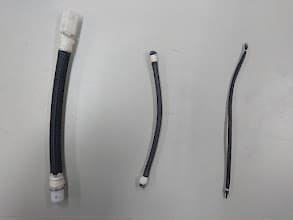
\includegraphics[scale=0.7]{image/hikaku.jpg}
  \caption{MPAの外径の比較(左から12,5,3 mm)}
  \label{fig:campare}
\end{figure}
%
\begin{figure}
  %
  \begin{minipage}{0.5\columnwidth}
    \centering  
    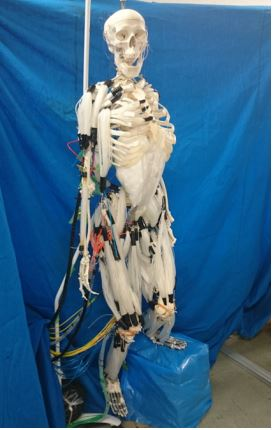
\includegraphics[scale=0.5]{image/kinkokkaku.JPG}
    \subcaption{筋骨格系ロボット\cite{森田隆介2016}}
    \label{fig:kin}
  \end{minipage}
  %
  \begin{minipage}{0.5\columnwidth}
    \centering
    \vspace{5mm}
    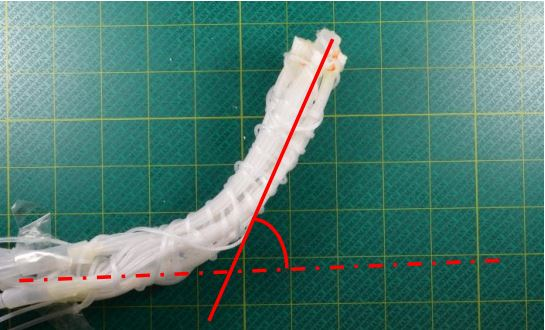
\includegraphics[scale=0.57]{image/takoJPG.JPG}
    \subcaption{タコ腕模倣メカニズム\cite{森和也2014}}
    \label{fig:tako}
  \end{minipage}
  %
  \caption{細径空圧筋を用いたロボット}
  \label{fig:saikei}
\end{figure}
  %
\begin{figure}[t]
  %
  \begin{minipage}{1\columnwidth}
    \centering
    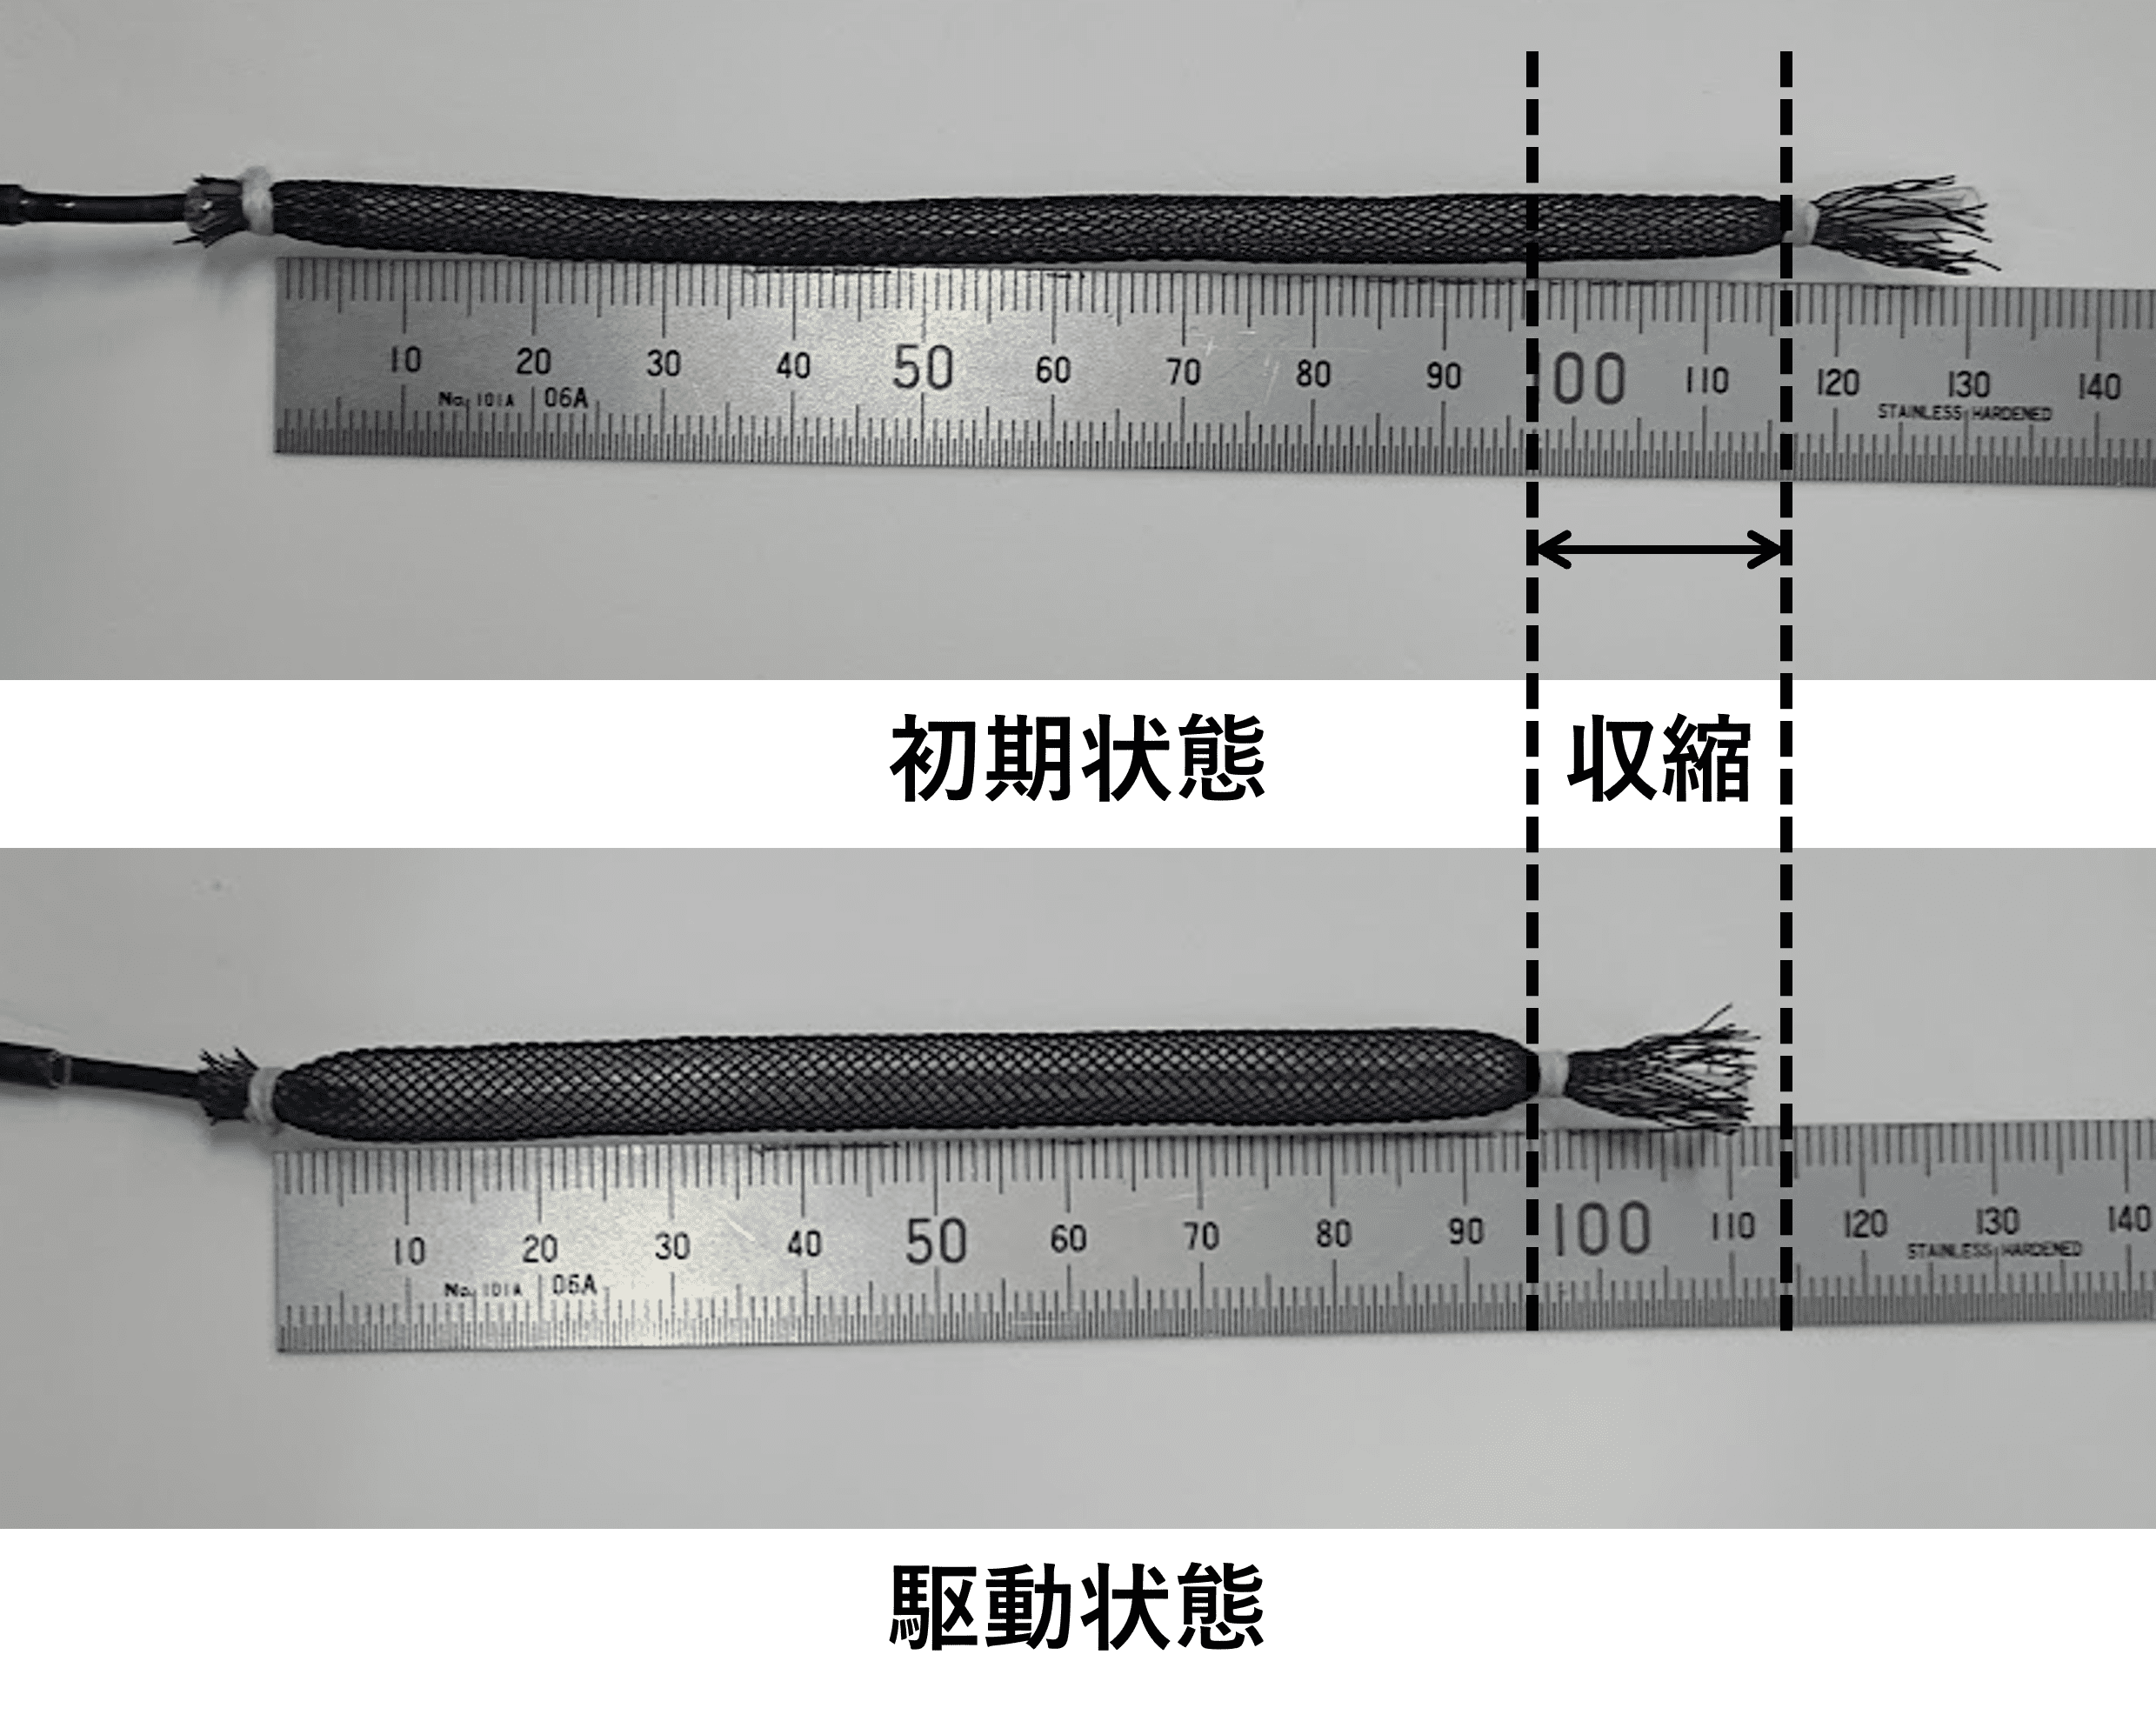
\includegraphics[scale=0.1]{image/syusyuku.png}
    \vspace{-3mm}
    \caption{収縮率}
    \label{fig:syusyuku}
  \end{minipage}
  %
  \begin{minipage}{1\columnwidth}
    \centering
    \vspace{3mm}
    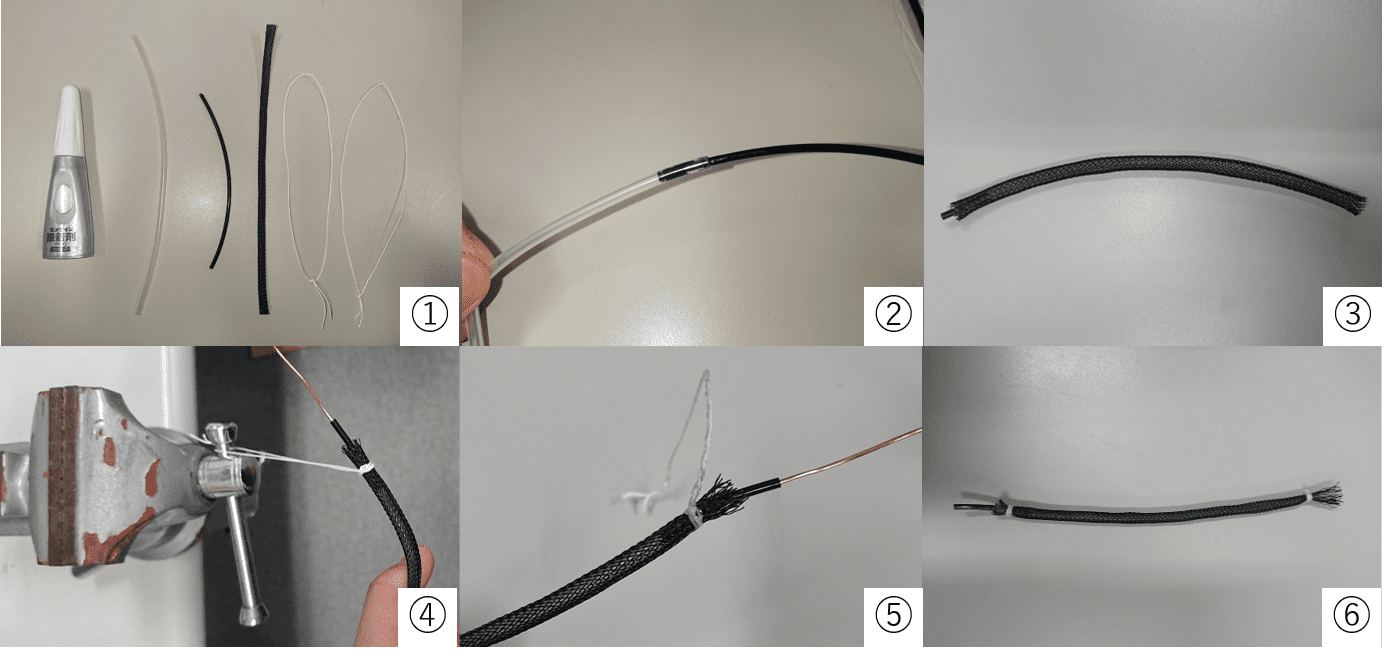
\includegraphics[scale=0.3]{image/method.png}
    \caption{細径MPAの作製手順}
    \label{fig:method}
  \end{minipage}
  %
\end{figure}
%
%%%%%%%%%%%%%%%%%%%%%%%%%%%%%%%%%%%%%%%%%%%%%%%%%%%%%%%%%
\subsection{細径MPAの作製方法}
本研究で用いる3 mmの細径MPAの作製方法について説明する.
構造は2.1節で述べた従来のMPAと同様,シリコンゴムチューブをナイロン繊維メッシュで覆ったシンプルなもので,0.4~0.5 MPaで駆動し収縮率は約18 %である(図\ref{fig:syusyuku}).
おおまかな作製手順を図\ref{fig:method}に示す.
端部の締結方法として端部に光造形方式の3Dプリンタで出力した部品を取り付ける方法(4.1.2節で使用)もあるが,ここでは直に紐で結び締結する手法を紹介する.
図中\textcircled{\scriptsize 1}に示した物品が作製に必要なもので左から以下の通りである.
%
\begin{itemize}
  \item PPX(瞬間接着剤) メーカー:セメダイン 品番:CA-522
  \item シリコンゴムチューブ 2×3(内径×外径) メーカー:タイガースポリマー 品番:SR1554
  \item ポリウレタンチューブ 2×1.2(外径×内径) メーカー:PISCO 品番:UB0212-20-B
  \item 編組チューブ 1×5(最小径×最大径) メーカー:モノタロウ 品番:-
  \item PEライン6号 (玉結びを2回し,長さ10 cmほどの輪っか状にしておく)
\end{itemize}
%
以下,作成手順である.
%
\begin{enumerate}
  \item まず初めにシリコンゴムチューブを任意の長さで切り,ポリウレタンチューブを1.5~2 cm幅で切る
  \item 切ったポリウレタンチューブをシリコンゴムチューブに約1 cm挿しこみ,挿しこんだ境界めがけて接着剤を塗布する(図中\textcircled{\scriptsize 2})
  \item 接着剤が十分に乾いたら編組チューブを被せる(図中\textcircled{\scriptsize 3})
  \item 3つのチューブが重なった部分をPEラインで結び,万力等に引掛け強く締結する(図中\textcircled{\scriptsize 4},締結方法については図\ref{fig:teiketu}参照).締結の際,締結部分の穴が塞がり圧縮空気を印加できなくなる恐れがあるためチューブ内に銅線等を挿しこんでおく
  \item 締結した部分に接着剤を塗布し,緩まないようにする(図中\textcircled{\scriptsize 5})
  \item 反対側も同様に締結し,接着剤を塗布することで完成する(図中\textcircled{\scriptsize 6})
\end{enumerate}
%
以上が本研究で用いる外径3 mmの細径MPAの作製手順である.
なお4.2.2節では端部に集積部品を取り付けているが,TPU等の柔らかい素材であれば同じ締結方法で締結できることが確認できているため,必要に応じて端部の形状は変更できる.
\begin{figure}[t]
  \centering
  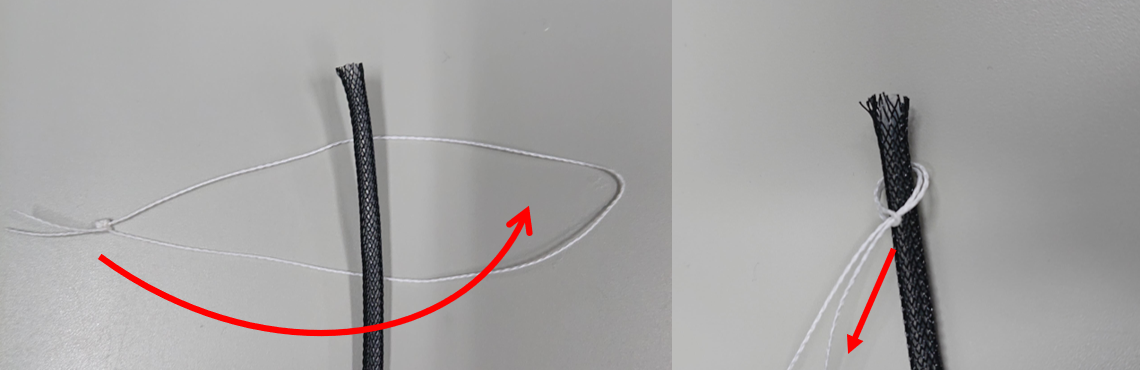
\includegraphics[scale=0.7]{image/teiketu.png}
  \caption{端部の締結方法}
  \label{fig:teiketu}
\end{figure}



